\section{Robot Vision Using a Pi Camera and OpenCV}
\label{robot_vision_using_pi_camera_opencv}

Giving a robot the ability to see things allows it to behave in ways to which humans relate
well. Computer vision is an area that much research is currently devoted to, but some of the
basics are already available for use in our own code, with the Pi Camera and a little bit of
work. In this section, we will use the robot and camera to drive to objects.

\begin{itemize}
\item Setting up a Raspberry Pi Camera on your robot, in terms of both software and hardware
\item Use Flask to create a web server to see what the robot sees on our laptop
\item Revisiting color models and learning how to mask images with them.
\item Using contours to detect the largest blob of color in an image and pointing the robot at it
\item Using Haar cascades to detect faces, and pointing the pan-and-tilt mechanism at them
\end{itemize}

\subsection{Set up the Raspberry Pi Camera}
We will first attach the camera to the pan-and-tilt assembly. We can then use a longer cable
to wire the camera into the Pi.

\subsection{Wire the Camera}
\label{wire_the_camera}

The Raspberry Pi has a slot specifically for the camera, the camera cable fits into this, see Figure \ref{raspberrypi_hdmi_csi}. We will be wiring our camera into this slot.

\begin{figure}[!htb]
\begin{center}
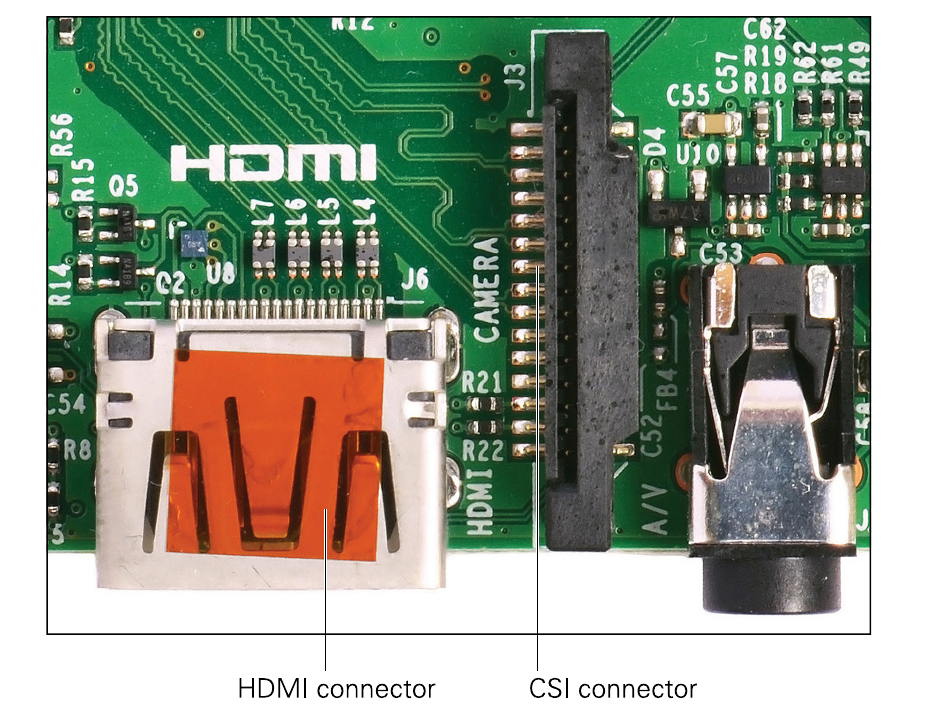
\includegraphics[scale=0.280]{img/raspberrypi/raspberrypi_hdmi_csi.jpeg}
\end{center}
\caption{ CSI and HDMI connectors.}
\label{raspberrypi_hdmi_csi}
\end{figure}

\begin{framed}
\begin{remark}{\textbf{Troubleshoot}}


See 

\url{https:/​/​www.​techcoil.​com/​blog/​connect-​raspberry-​pi-​camera-​module-​raspberry-​pi-2-​raspberry-​pi-​3/}
on how to connect the raspberry pi camera module using the long 300 mm cable. 
\end{remark}
\end{framed}

\subsection{Activate the Camera}
\label{activate_camera}

In this section, we will set up the camera, activating it in Raspbian and getting a test
picture. 

Power up the Pi on external power (that is, plugged into a USB wall adapter) for this
operation,  and log in via PuTTY. At the Terminal, type the following:

\begin{lstlisting}
sudo raspi-config
\end{lstlisting}

In \lstinline{raspi-config}, select the \textbf{5 Interfacing Options} option,and then select P1 Camera. 
You will then be asked if you would like the camera interface to be enabled. Select Yes and Ok, then Finish. 
If you are asked to reboot at this point, answer Yes. 


\subsubsection{Get a Picture from the Pi Camera}
\label{get_a_picture}

Now that we enbled the camera, the first thing we need to do, is to confirm that our setup was successful.
Thus, we will use the Pi camera to take a picture for us. This will check whether all the connections are good or not.
If there are problems detecting the camera, please go back and check that the cable
connection is correct, that you have installed picamera, and that you have enabled the
Raspberry Pi camera in \lstinline{raspi-config}.

Reconnect to the Raspberry Pi with PuTTY, and type the following to get a picture:

\begin{lstlisting}
raspistill -o test.jpg
\end{lstlisting}

\lstinline{raspistill} takes a still image, and the \lstinline{-o} parameter tells it to store that image in
\lstinline{test.jpg}. 

We can use the FileZilla client (see appendix) to download this image and verify it on our computer. 


\subsection{Setting up OpenCV, NumPy and PiCamera}
\label{setup_opencv}

In this section, we will install the OpenCV, \url{https://opencv.org/}, library  on the Rasperry Pi. In case you do not know OpenCV, this 
is  a library with a collection of tools for manipulating pictures and extracting
information from them. The name is an abbreviation of Open Computer Vision. The tools are
strung together to make useful behaviors and pipelines for processing images. To be able to
run our code on the Raspberry Pi, we will need to install the Python OpenCV library there.

We will also install NumPy, \url{http://www.numpy.org/}, the numeric python library. This lets us to do manipulations of
large blocks of numbers. 

Finally, we will install PiCamera. \url{https://picamera.readthedocs.io/en/release-1.13/}, a library for manipulating our Pi camera.


\subsubsection{Install NumPy}

We can install NumPy using \lstinline{pip}

\begin{lstlisting}
pip3 install numpy
\end{lstlisting}

\subsubsection{Install OpenCV}

We can install OpenCV via terminal

\begin{lstlisting}
sudo apt install python-opencv opencv-data
\end{lstlisting}

\begin{framed}
\begin{remark}

Have a look at the following links should you have problems in setting up OpenCV in Raspberry Pi
\url{https://blog.piwheels.org/how-to-work-out-the-missing-dependencies-for-a-python-package/}
\end{remark}
\end{framed}

\subsubsection{Install PiCamera}

Finally, we will install the PiCamera library so that we can interact with the Pi camera

\begin{lstlisting}
sudo pip3 install picamera[array] numpy
\end{lstlisting}

\section{Building a Flask Web Server}

Downloading one picture at a time is fine, but we actually need to be able to do things with
those pictures on the robot. We also need a handy way to see what the robot is doing with
the camera data. For that, we will reach back into our toolkit, and use a Flask web server to
serve up our pictures. We can use the core of this app to make a few different behaviors.
We'll keep the base app around for them.

Figure \ref{server_app} shows a pipeline, with our image data going from the camera,
through the pipeline, and out to our web browser. The process image step can be anything
we require; for this example, we'll apply a color mask, which we explore in more depth in
the next section:

\begin{figure}[!htb]
\begin{center}
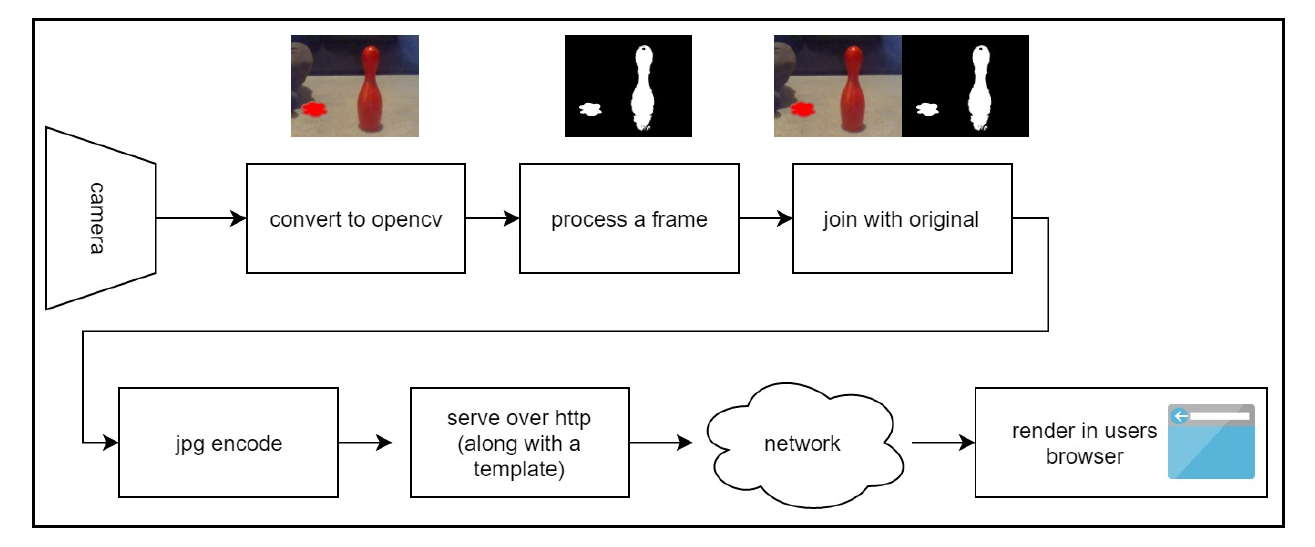
\includegraphics[scale=0.280]{img/raspberrypi/server_app.jpeg}
\end{center}
\caption{The image server app.}
\label{server_app}
\end{figure}

It's time to start building the code to do this. Because this is fairly complex, we'll break it
down into two major parts: first, a \lstinline{CameraStream} object, which will send our frames to an
\lstinline{image_server.py} script, the second part of our code project.




